Matt Iverson

2014-10-07

Writing essay for the EKOCYCLE 3D printer application

\begin{tabular}{|p{5cm}|p{5cm}|}
 \hline
 What you did this week: &
 Reflections: \\
 \hline
 Calculated the space we’d need for a scissor lift / conveyor belt mechanism. &
 The mechanism will fit and reach high enough, but it’ll take up a lot of space. \\
 \hline
\end{tabular}

I’ve been writing the essay for the last day and a half. Not exactly what I expected to be doing on a robotics team, but a 3D printer would be extremely useful for us. I’m still working on the first draft; writer’s block is setting in like always. This is what the printer looks like:

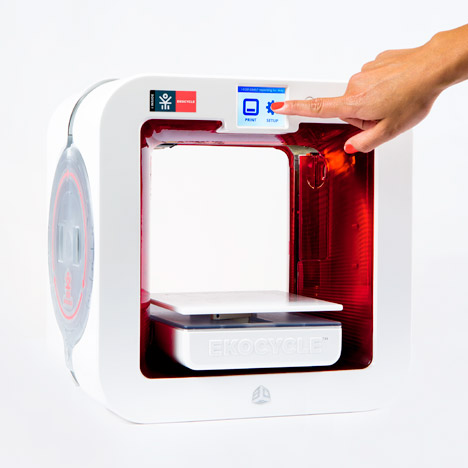
\includegraphics[width=10cm]{./Entries/Images/ekocycle.jpg}
